\clearpage
\chapter{Detailed Design}
\section{UML Diagrams}

\subsection{Use Case Diagrams}
\begin{figure}[!htbp]
    \centering
    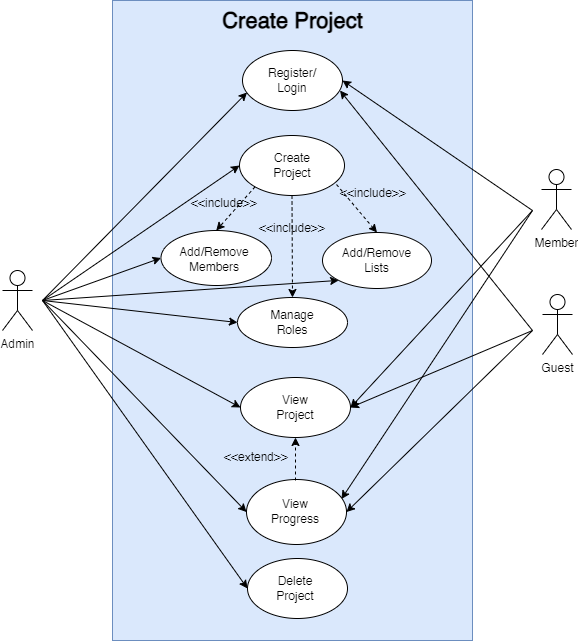
\includegraphics[width = 0.8\textwidth]{createproject.png}\\[0.1in]
    \caption{Create Project}
    \label{fig:my_label}
\end{figure}
The Actors are Admin, Member and Guest. Admin will do the functions like create/delete project, add/remove members to the project, manage roles etc. Member can login, view the project and view progress. The guest/client can view the project and it's progress.
\FloatBarrier

\begin{figure}[!htbp]
    \centering
    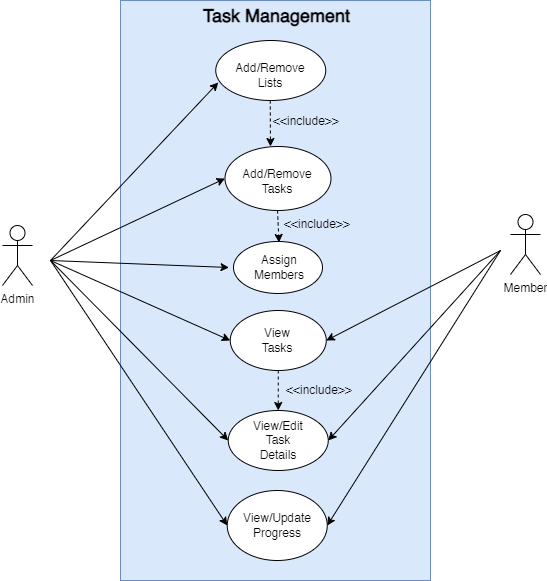
\includegraphics[width = 0.8\textwidth]{Tasksmngmnt.png}\\[0.1in]
    \caption{Task management}
    \label{fig:my_label}
\end{figure}

\FloatBarrier

\subsection{Class Diagrams}
\begin{figure}[!htbp]
    \centering
    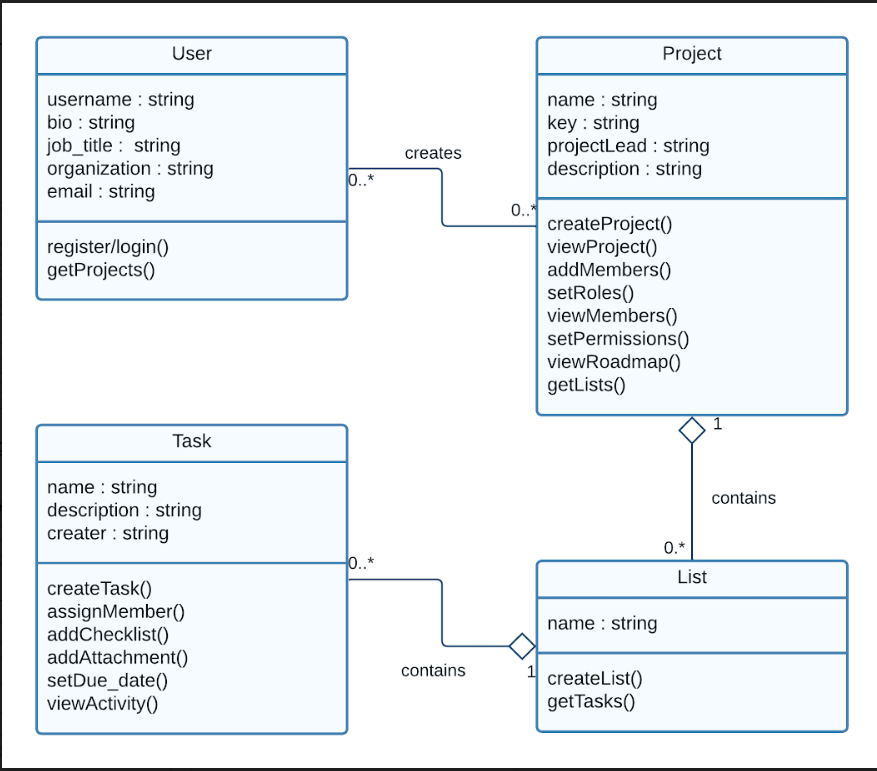
\includegraphics[width = 0.8\textwidth]{classdiagram.png}\\[0.1in]
    \caption{Class Diagram}
    \label{fig:my_label}
\end{figure}

\FloatBarrier
 
\subsection{Sequence Diagrams}

\begin{figure}[!htbp]
    \centering
    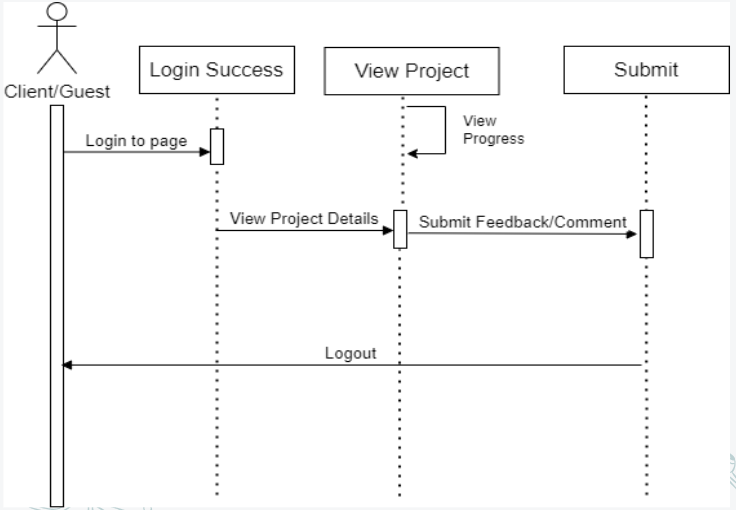
\includegraphics[width = 0.8\textwidth]{seqDgmClnt.png}\\[0.1in]
    \caption{Sequence Diagram for Client}
    \label{fig:my_label}
\end{figure}

\begin{figure}[h]
    \centering
    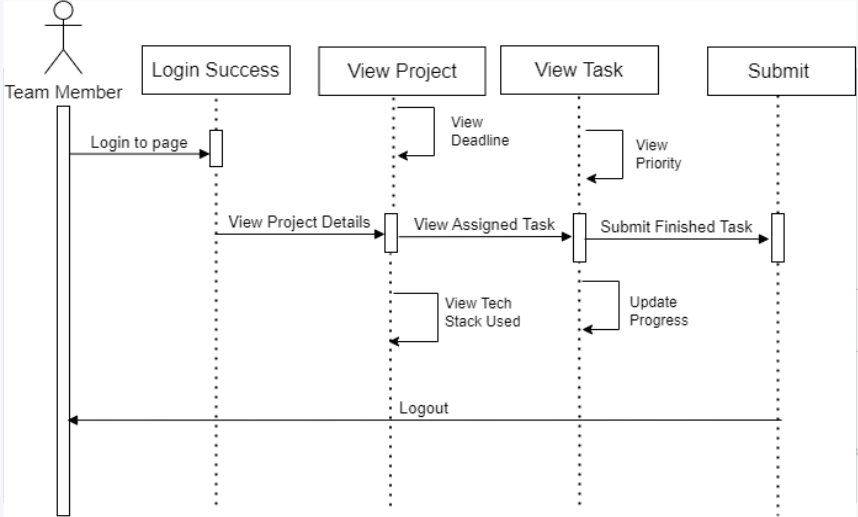
\includegraphics[width = 0.8\textwidth]{seqDiagramTeamMem.png}\\[0.1in]
    \caption{Sequence Diagram for Team members}
    \label{fig:my_label}
\end{figure}


\FloatBarrier

\subsection{Activity Diagrams}

\begin{figure}[!htbp]
    \centering
    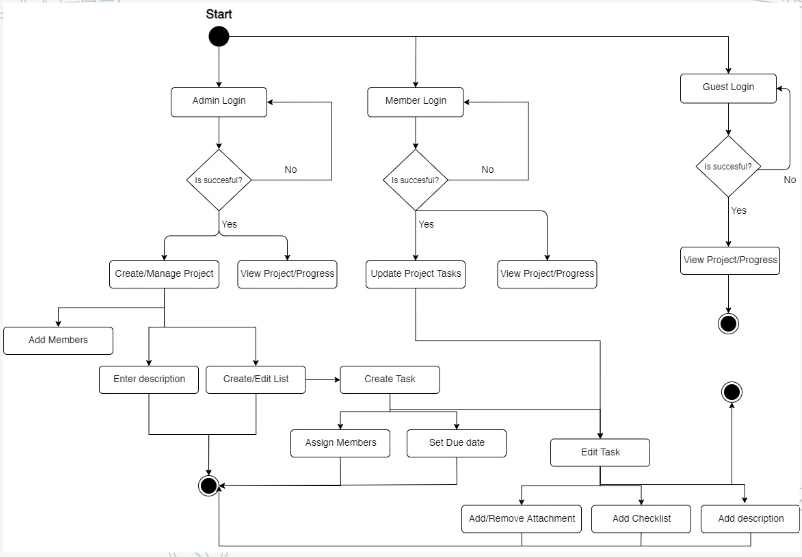
\includegraphics[width = 0.8\textwidth]{actvDgm.png}\\[0.1in]
    \caption{Activity Diagram}
    \label{fig:my_label}
\end{figure}



